%!TEX root = ../report.tex

\begin{document}
    \chapter{State of the Art}
    \label{chap:State of the Art}
    Point cloud registration algorithms are normally classified into two major categories: global (coarse) registration and local (fine) registration \cite{Quan_2020_com,Kim_2011_fully}.
    Coarse registration algorithms attempt to find a transformation that approximately maps the source point cloud to the target point cloud. 
    Fine registration algorithms attempt to refine an initial transformation to map the source point cloud to the target point cloud.
    There are some approaches that combine both of these methods, they first apply a global method and then refine the results with the help of a local method. 
    We can classify these approaches into a 3rd category of hybrid methods. 
    \par
    
    For the purpose of this work we can classify point cloud registration algorithms into two major categories:
    point-to-point and point-to-model.
    Point-to-point registration algorithms attempt to align two point clouds, while point-to-model registration algorithms attempt to align a point cloud with a 3D model.

    The approaches that do not work with point cloud data or 3D models, but are still related to the registration problem, are classified into the category of others.

    \begin{figure}[H]
        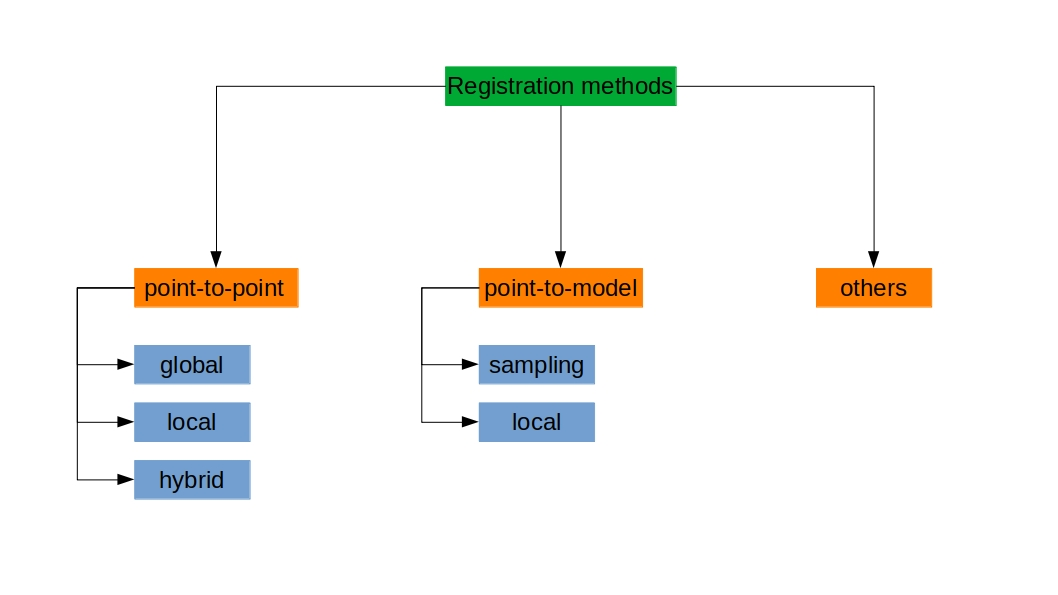
\includegraphics[width=\textwidth]{images/Classification.jpg}
        \caption{Classification of the State of the Art.}
        \label{fig:classification}
    \end{figure}

    Figure \ref{fig:classification} shows an overview of the papers reviewed.



    \section{Point-to-point registration}

        \subsection{Global methods}

        RANSAC \cite{Fischler_1981_RANSAC} can also be used to perform the registration task but is time-consuming due to the randomness
        of the RANSAC algorithm. Therefore, Pankaj et al. \cite{Pankaj_2015_arobust} present a guided sampling improvement to RANSAC,
        to reduce the registration time, sorting the correspondences obtained from a previous 3D feature matching according to its quality.
        
        Following the same line, S. Quan and J. Yang \cite{Quan_2020_com} propose a method that helps the RANSAC algorithm 
        sampling the best point correspondences. Their approach first detects keypoints using Harris3D, then it matches the keypoints
        by using the Local Voxelized Structure (LoVS) descriptor. After that, the set of correspondences is reduced using the 
        Nearest Neighbor Similarity Ration (NNSR) and the compatibility score of the remaining correspondences with the rigidity and 
        DSP constraint. Finally, the correspondences with the best compatibility scores are using to generate transformations and 
        the best one (the one with the maximum number of inliers) is the final result. Unfortunately, the RANSAC-based approaches are sensitive to outliers.

        Another less common approach for coarse registration is proposed by Sakakubara et al. \cite{Sakakubara_2007_automatic}.
        This coarse registration approach uses Mixed Integer Linear Programming to find pairs of corresponding points that are then 
        used to find a coarse transformation that aligns two different point clouds.
        This approach finds a global optimal result without using the values of the invariant features, 
        it adjusts the error tolerance depending on the accuracy of the given data and 
        it finds the best correspondences between the points.
        Nevertheless, Mixed Integer Linear Programming problems are NP-hard. Therefore, this approach is excessively time-consuming.

        Others have proposed the use of neural networks to attempt to solve the global registration problem.
        This is the case of Wang and Solomon \cite{Wang_2019_deepclosest}. They propose a learning-based method called Deep Closest Point (DCP).
        The approach proposed first uses PointNet \cite{Qi_2017_pointnetdeep} or DGCNN \cite{Wang_2019_dynamic} to embed the point clouds.
        Then, it uses an attention-based module to encode the output of the first part.
        Finally, it estimate the transformation using a differentiable SVD layer.

        Sarode et. al \cite{Sarode_2019_oneframework} present a registration framework that also use the PointNet to extract feature from the point clouds.
        The PointNet features are then aligned using another network. The process is then repeated a given number of times to improve the registration result.
        
        Ding and Feng \cite{Ding_2019_deepmapping} present another deep learning method called DeepMapping,
        whose main structure is constituted of two deep neural networks.
        The first network is a localization network, whose output is the pose estimation for the input point clouds.
        And the second network is a map network that estimates the occupancy status of the input locations to compute a loss function that reveals
        the registration quality.

        More recently, Huang et al. \cite{Huang_2020_feature} propose a learning method that can be trained in a semi-supervised or unsupervised way.
        The proposed framework is composed of an encoder, that extracts features from the input point clouds, 
        and a decoder that decodes the extracted features to compute a projection error that serves as input for an algorithm that estimates
        a transformation increment. 
        This increment is then employed to update the parameters of the transformation and transform one of the point clouds.
        The whole process is repeated until the loss computed is less than some desired value.
    


        \subsection{Local methods}

        Besl and N. D. McKay \cite{Besl_1992_amethod} propose the Iterative Closest Point (ICP) algorithm to perform registration 
        between point sets, line segments, implicit curves, parametric curves, triangles, implicit surfaces, and parametric surfaces.
        ICP iteratively finds and updates correspondences between the desired sets based on an initial approximation to the solution and 
        the spatial distance.

        According to Segal et al. \cite{Segal_2009_generalizedicp}, the ICP algorithm can be summarized in two main steps:
        the computation of correspondences between the two scans and 
        the computation of a transformation that minimizes the distance between corresponding points.
        They present a generalized version of the ICP algorithm by attaching a probabilistic model to the second step.
        This generalization makes the algorithm more robust to outliers without modifying the simplicity. 
        However, it does not improve the speed of the original ICP.

        ICP and its variants are still the standard algorithms for point cloud registration because of their simplicity. 
        % Nevertheless, to perform well they require a good initial approximation of the solution.

        \subsection{Hybrid methods}

        The results of the global methods can be refined with the use of a local method, most of the time a variation of the popular ICP.
        In this category, some of these methods can be found.

        Go-ICP is a branch-and-bound (BnB) based approach proposed by Yang et al. \cite{Yang_2016_goicp} to address the susceptibility of ICP to local minima. 
        The main idea of Go-ICP is that BnB and ICP work iteratively until a global minimum is reached: BnB finds a solution and this is refined by ICP.
        Go-ICP guarantees global optimality regardless of the initialization and it is recommended for scenarios where real-time performance is not critical.

        The approach proposed by Jun Lu et al. \cite{Lu_2019_4pcsicp} obtains a consistent four-point set by using Super4PCS \cite{Mellado_2014_super4pcs}, 
        then it creates a neighborhood ball with each point as the center and obtains the overlapping regions as the intersections
        of these neighborhood balls. Finally, ICP is applied to the overlapping regions. The main drawback of this method is that 
        there should exist overlapping regions in order to perform the registration task.

        Because of the increasing success of Deep Learning in 2D applications, there have been attempts to use deep neural networks
        to solve the complete point cloud registration problem (global and local registration).
        DeepICP \cite{Lu_2019_deepicp} is the first end-to-end learning-based point cloud registration framework.
        DeepICP makes use of other networks to build a complete framework.
        The first step of DeepICP is the Deep Feature Extraction (PointNet++ \cite{Qi_2017_pointnet}), which extracts features from the point clouds.
        In the second step, the Pont Weighting (3DFeatNet \cite{Yew_2018_3dfeat}) selects the relevant points.
        In the third step, the selected points of the target point cloud are sampled using the initial transformations.
        In the fourth step, Deep Feature Embedding is used to obtain more specific descriptors of the points.
        In the final step, the corresponding pair of points are generated with a 3D Convolutional Neural Network
        to compute an improvement of the initial transformation.
        
        Another approaches does not use a neural network to solve the complete point cloud registration problem but a part of it.
        LORAX is an algorithm proposed in \cite{Elbaz_2017_3dpoint} that selects some sets of points called super-points and uses a low-dimensional descriptor 
        generated by an autoencoder to describe the structure of each super-point.
        The sets of superpoints of both pointclouds are then matched using the euclidean distance between the descriptors.
        Finally, a coarse registration is computed using a RANSAC procedure, followed by a fine registration using ICP.
        The main contribution of LORAX is the use of an autoencoder to extract features of 3D point clouds. 
        Nevertheless, the implementation is not optimized for real-time performance and it is not proved to be fast for big point clouds.

    \section{Point-to-model registration}

        \subsection{Sampling methods}

        In order to register a 3D model with a point cloud, the simpliest idea is to sample points from the 3D model to generate a second point cloud
        and then perform one of the point-to-point registration methods. 

        Kim et al. \cite{Kim_2011_fully} register a 3D CAD model of a construction site with a point cloud by sampling points from the 3D model 
        and then applying a point-to-point registration algorithm. The registration consists of three main steps. First, 
        the point clouds are re-sampled to the same resolution. Second, PCA is used to identify the principal axes of the data 
        to obtain a coarse registration based on these axes. Third, fine registration is performed with the Levenberg-Marquardt
        iterative closest point (LM-ICP) algorithm \cite{Fitzgibbon_2003_robust}. 
        
        Kim et al. \cite{Kim_2013_fully} is an extension of their previous work \cite{Kim_2011_fully}
        In this approach, they just add a noise filter step to the pre-processing of the point cloud in order to improve the registration results.
        The rest of the steps remain the same.
        However, using PCA for coarse registration will not assure a good performance when the form of the building is close to a cube.
        
        \subsection{Local methods}

        Other approaches work directly with the information provided in the 3D models to perform the registration task.

        Li and Song \cite{Li_2015_amodified} propose two extensions to the most popular local registration method, the ICP algorithm, 
        to be able to use it with an STL-file (3D model) and a point cloud.
        The first of these extensions is called ICP-STL, and its main modification consists of finding the corresponding triangle mesh of the STL file of the points 
        in the point cloud, and then the closest point in the triangle mesh to each point of the point cloud. The rest of the ICP algorithm remains the same.
        The second modification is called ICP-DAF (ICP dynamic adjustment factor), and it aims to reduce the time of the ICP-STL method. 
        ICP-DAF adds a dynamic adjustment factor to adjust the transformation parameters dinamically.
        The disadvantage of this method is the same disadvantage present in the ICP algorithm, to perform well it requires a good initial approximation of the solution.

        In the specific case of CityGML, Goebbels et al. \cite{Goebbels_2019_icpcitygml} propose an extension of the well-known ICP
        to perform point-to-model registration based on the point-to-plane registration.
        This approach only considers points on the perimeter of the buildings.
        The main contribution of this approach is the speed. Point-to-model ICP is faster than the point-to-plane ICP.
        Nevertheless, CityGML models used do not contain terrain information. 
        Therefore, the ground plane is the lowest point of the building and some walls might intersect with the real terrain, increasing the error of the algorithm.
        An additional disadvantage of this method is that it expects the point cloud to be coarsely register with the model.

        Another approach by Goebbels et al. \cite{Goebbels_2018_linebased} explores the possibility to find features that help to perform the registration.
        The approach first rotates the point cloud to align the walls to the z-axis. Then it projects all the points onto the 
        xy-plane to obtain a 2D image of the point cloud viewed from above. After that, it detects the corners or lines in the 2D image,
        and having the corners or lines of the CityGML model it applies a Mixed Integer Linear Program to perform the registration.
        Nonetheless, the point cloud has to be already coarsely registered in order to obtain a successful and fast result.

        An extension of the work in \cite{Goebbels_2018_linebased} has been made by Goebbels et al. \cite{Goebbels_2018_alinear}, 
        where the steps to perform the registration are the same.
        However, in the last step, a Linear Program is used to fine-tune the coarse result. 
        Unfortunately, the results of this method depend on the value of an error bound, which affects the generalization of the algorithm.
        Moreover, it has the same disadvantage as the previous approach: 
        the point cloud has to be already coarsely registered in order to obtain a successful and fast result.

        
    \section{Others}
    There are other approaches that attempt to solve different matching problems with or without correspondences.
    These approaches cannot be classified in the previous categories because their input data is not composed of two point clouds or one point cloud and a 3D model.
    Some of these approaches are collected into this category.

    Breuel \cite{Breuel_2003_implementation} proposes the use of matchlist-based BnB techniques to solve geometric matching problems without correspondences.
    For example, point and line segment matching in 2D and 3D.

    Bazin et. al \cite{Bazin_2013_abranchandbound} present an approach that combines Linear Programming and BnB procedures to achieve global optimality.
    The proposed algorithm receives two different sets of features extracted from two images and outputs
    the correspondences between the features verifying the appearance similarity and geometric constraints.
    In the end, it not only computes the feature correspondences but also computes an estimation of a geometric transformation between the features
    and identifies the inliers/outliers.

    Brown et. al \cite{Brown_2015_globally} extend the idea of the two previous approaches and present a 2D-3D registration method that does not need
    correspondences, by using a BnB algorithm. They also propose a deterministic annealing algorithm to reduce computation time.
    The proposed method works with points or lines, but not with a combination of both.
    Therefore, Brown et. al \cite{Brown_2019_afamily} propose a framework to solve the 2D-3D registration problem without feature correspondences
    that is able to use points, lines, or a combination of both.

    Windheuser et al. \cite{Windheuser_2011_largescale} propose the use of Integer Linear Programming to find correspondences between non-rigid 3D shapes.
    They use an Integer Linear Program to minimize the elastic thin-shell energy requires to deform one shape into the other one.
    Their method can be improved by a relaxation of the Integer Linear Program and by including feature descriptors.

    \section{Limitations of previous work}
    ICP and its variants provide simple and easily-implemented iterative methods, but these algorithms can converge to false local optima \cite{Wang_2019_deepclosest}.
    Furthermore, they do not scale well with the number of points and they are not differentiable, therefore they cannot be integrated into end-to-end
    deep learning pipelines \cite{Sarode_2019_oneframework}. 
    And the principal disadvantage of these methods is that they require a good initial approximation to the solution to perform well.
    
    RANSAC and its variations cannot guarantee any global optimality in their final results \cite{Bazin_2013_abranchandbound}.
    According to \cite{Quan_2020_com}, RANSAC has two main issues. 
    The first one is its computational complexity, which makes it time-consuming.
    The second one is its randomness during sampling that can lead to inaccurate results.
    These two disadvantages worsen with the number of outliers.

    The globally optimal methods such as Linear programming and BnB based methods are very time-consuming. 
    Therefore, their application in real-time tasks is limited \cite{Sarode_2019_oneframework}.

    In the last years, there has been a boom in the use of neural networks and deep neural networks to solve 2D problems.
    Therefore, their use in 3D tasks has been explored too.
    Unfortunately, methods based on deep learning generally suffer from issues regarding the generalization ability and the requirement of massive training data \cite{Quan_2020_com}.

    In general, one thing that can be noticed is that none of this methods offers a direct solution for the coarse registration of a model with a point cloud.
    The only solution available for this is to sample a point cloud from the model and apply a global method for two point clouds.
    Unfortunately, this solution does not leverage the complete information contained in the model.

\end{document}
